% ------------------------------------------------------------- 
% Arquivo :  relatório modelo                                        
% ------------------------------------------------------------- 
% O percentual(%) serve para incluir comentários: 
% tudo o que fica à direita dele não é interpretado pelo LaTex
% Linhas e espaços em branco também **NÃO** são
% interpretadas pelo LaTex

%% As intruções seguintes são o cabeçalho e devem estar antes do
%% \begin{document}

%\documenclass: mandatorio, indica o tipo/formato de documento
\documentclass[brazilian,12pt,a4paper,final]{article}
% tamanhos de fontes: 10pt, 11pt ou 12pt
% opções de estilo (padrões): article, report, book, slide, letter (artigo, relatorio, livro, apresentação de slides, carta)




%% Pacotes extras (opcionais):

% *babel* contem as regras de ifenização
\usepackage[brazil]{babel}

% *t1enc* permite o reconhecimento dos acentos inseridos com o teclado
%\usepackage{t1enc}

% *inputenc* com opção *utf8* permite reconhecimento dos caracteres com codificação UTF8, que é padrão dos esditores de texto no Linux. Isso permite reconhecimento automático de acentuação.
\usepackage[utf8]{inputenc}


% *graphicx* é para incluir figuras em formato eps 
\usepackage{graphicx} % para produzir PDF diretamente reescrever esta linha assim: \usepackage[pdftex]{graphicx}

% *color* fontes soloridas
\usepackage{color}
%%% fim do cabecalho %%%

\pagestyle{empty}
\title{Trabalho1 : Movimento Browniano}
\author{Aluno: Leonardo Machado Barcelos - Matrícula: 00302060 \\ IF-UFRGS}

\begin{document}
\maketitle
\begin{abstract}
Dados de deslocamento quadrático médio com o tempo.
% as quebras de linha coma a de cima não são interpretadas
% para forzar quebra de linha deve ser deixada uma linha em branco
\end{abstract}

%Abaixo podem ver como se deve colocar letras acentuadas ou latinas se
%o pacote *t1enc* não dfosse usado 
\section{Movimento Browniano} 

\begin{figure}[hbtp]
\begin{center}
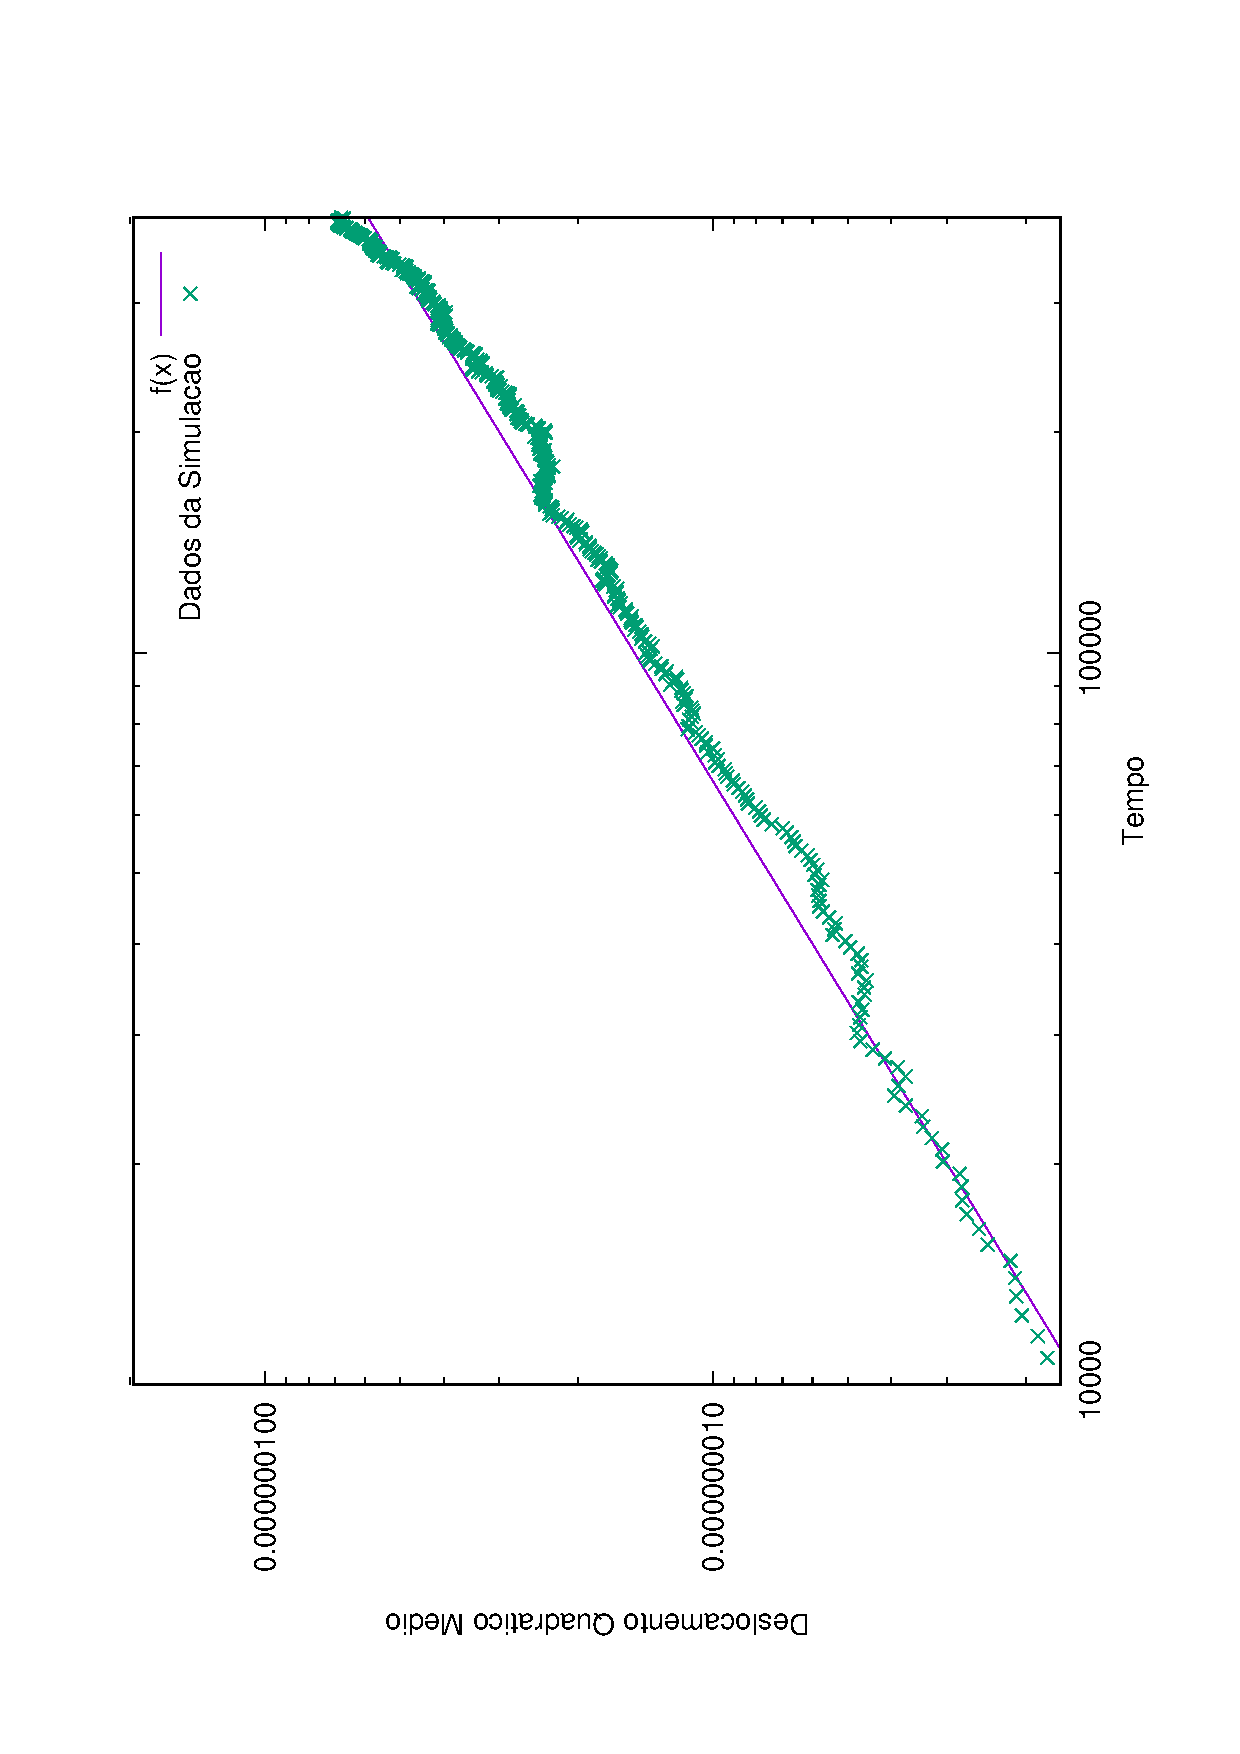
\includegraphics[width=12cm]{browniano.pdf}
\caption{Brownianas}
\label{fig}
\end{center}
\end{figure}

% Aqui a Introdução \c{c} e \~a  é a forma standar  de escrever
% carateres ASCII extendidos (acentos, etc), porem com o pacote t1enc
% declarado acima podemos escrever diretamente ç em lugar d \c{c}, etc
O Deslocamento quadrático médio, do inglês \emph{Mean square displacement} ($MSD$), é uma medida da capacidade de dispersão (difusão) das partículas no sistema. Ela representa a média dos quadrados dos deslocamentos em relação à uma posição anterior de referência de cada partícula (Note que a média dos deslocamentos das partículas é nula, pois o centro de massa não se move, por isso a necessidade de tomarmos os quadrados). Matematicamente, podemos expressar:

$$MSD = \langle (\vec{r} - \vec{r_0})^2 \rangle = \frac{1}{N} \sum_{i=1}^{N}(x_i(\Delta{t}) - x_0_i)^2 +  (y_i(\Delta{t}) - y_0_i)^2$$

Perceba que o $MSD$ é uma função do tempo (na verdade, do intervalo de tempo) e portanto estamos interessados em estudar como esta função varia no tempo. Em dinâmicas com fases líquidas e gasosas, teremos então o fenômeno da dispersão. As partículas irão "caminhar" por todo o espaço permitido em um movimento aleatório. Este movimento é conhecido como movimento Browniano e fui estudando por grandes cientistas, como Albert Einstein.

\begin{thebibliography}{99}

\bibitem{Kauffman_book}
S.~Kauffman, {\em The Origins of Order: Self-Organisation and
Selection in Evolution}, (Oxford University Press, 1993).

\bibitem{Wolfram_book}
S.~Wolfram, {\em Theory and Application of Cellular Automata},
(World Scientific, Singapore, 1986).

\end{thebibliography}

\end{document}

